\documentclass{beamer}

\usepackage{amssymb,amsmath,amsfonts,graphicx}
\usepackage[english]{babel}
\usepackage{graphics}
\usepackage{beamerthemesplit} 
\usepackage{beamerthemeshadow}
\usepackage[latin1]{inputenc}
\usefonttheme{professionalfonts}
\usepackage{times}
\usepackage{amsmath}
\usecolortheme{whale}
\usepackage{enumerate}
\usepackage{amssymb}
\setcounter{tocdepth}{3}
\usepackage{graphicx}
\usepackage{times}
\usepackage{subfigure}
\usepackage{color}
\usepackage{amsbsy}
\usepackage{amsmath}
\usepackage{amsfonts}
\usepackage{amssymb}
\usepackage{epsfig}
\usepackage{tabulary}
\usepackage{wrapfig}
\usepackage[noadjust]{cite}

%%%%%%%%%%%%%%%%%%%%%%%%%%%%%%%%%%%%%%%%%%%%%%%%%%%%%%%%%%%%%%%%%%
% General
%%%%%%%%%%%%%%%%%%%%%%%%%%%%%%%%%%%%%%%%%%%%%%%%%%%%%%%%%%%%%%%%%%
\newfont{\msym}{msbm10}
\newcommand{\reals}{\mathbb{R}}%Re}%{mbox{\msym R}}
\newcommand{\half}{\frac{1}{2}}       
\newcommand{\sign}{{\rm sign}}
\newcommand{\paren}[1]{\left({#1}\right)}
\newcommand{\brackets}[1]{\left[{#1}\right]}
\newcommand{\braces}[1]{\left\{{#1}\right\}}
\newcommand{\ceiling}[1]{\left\lceil{#1}\right\rceil}
\newcommand{\abs}[1]{\left\vert{#1}\right\vert}
\newcommand{\tr}{{\rm Tr}}
\newcommand{\pr}[1]{{\rm Pr}\left[{#1}\right]}
\newcommand{\prp}[2]{{\rm Pr}_{#1}\left[{#2}\right]}
\newcommand{\Exp}[1]{{\rm E}\left[{#1}\right]}
\newcommand{\Expp}[2]{{\rm E}_{#1}\left[{#2}\right]}
\newcommand{\eqdef}{\stackrel{\rm def}{=}}
\newcommand{\comdots}{, \ldots ,}
\newcommand{\true}{\texttt{True}}
\newcommand{\false}{\texttt{False}}
\newcommand{\mcal}[1]{{\mathcal{#1}}}
\newcommand{\argmin}[1]{\underset{#1}{\mathrm{argmin}} \:}
\newcommand{\normt}[1]{\left\Vert {#1} \right\Vert^2}
\newcommand{\step}[1]{\left[#1\right]_+}
\newcommand{\1}[1]{[\![{#1}]\!]}
\newcommand{\diag}{{\textrm{diag}}}
%\newcommand{\det}{{\textrm{det}}}
\newcommand{\KL}{{\textrm{D}_{\textrm{KL}}}}
\newcommand{\IS}{{\textrm{D}_{\textrm{IS}}}}
\newcommand{\EU}{{\textrm{D}_{\textrm{EU}}}}
\newcommand{\lloss}{\ell} % label loss
\newcommand{\closs}{\hat\ell} % classifier loss
\newcommand{\st}{\textrm{s.t.}} % such that / subject to

%%%%%%%%%%%%%%%%%%%%%%%%%%%%%%%%%%%%%%%%%%%%%%%%%%%%%%%%%%
% Control symbols
%%%%%%%%%%%%%%%%%%%%%%%%%%%%%%%%%%%%%%%%%%%%%%%%%%%%%%%%%%
\newcommand{\leftmarginpar}[1]{\marginpar[#1]{}}
\newcommand{\figline}{\rule{0.50\textwidth}{0.5pt}}
\newcommand{\pseudocodefont}{\normalsize}
\newcommand{\nolineskips}{
\setlength{\parskip}{0pt}
\setlength{\parsep}{0pt}
\setlength{\topsep}{0pt}
\setlength{\partopsep}{0pt}
\setlength{\itemsep}{0pt}}

%%%%%%%%%%%%%%%%%%%%%%%%%%%%%%%%%%%%%%%%%%%%%%%%%%%%%%%%%%%
% Equations and references
%%%%%%%%%%%%%%%%%%%%%%%%%%%%%%%%%%%%%%%%%%%%%%%%%%%%%%%%%%%
\newcommand{\beq}[1]{\begin{equation}\label{#1}}
\newcommand{\eeq}{\end{equation}}
\newcommand{\beqa}{\begin{eqnarray}}
\newcommand{\eeqa}{\end{eqnarray}}
%\renewcommand{\eqref}[1]{Eq.~(\ref{#1})}
\newcommand{\exmref}[1]{Example~\ref{#1}} 
\newcommand{\sthmref}[1]{Thm.~\ref{#1}}  
\newcommand{\remref}[1]{Remark~\ref{#1}} 
\newcommand{\claimref}[1]{Claim~\ref{#1}} 
\newcommand{\corref}[1]{Corollary~\ref{#1}} 
\newcommand{\scorref}[1]{Cor.~\ref{#1}} 
\newcommand{\tran}[1]{{#1}^{\top}}
\newcommand{\norm}{\mcal{N}}
\newcommand{\eqsref}[1]{Eqns.~(\ref{#1})}

% Alex's macros

\newcommand{\chaplabel}[1]{\label{chap:#1}}
\newcommand{\chapref}[1]{Chapter~\ref{chap:#1}}

\newcommand{\seclabel}[1]{\label{sec:#1}}
\newcommand{\secref}[1]{Section~\ref{sec:#1}}

\newcommand{\applabel}[1]{\label{app:#1}}
\newcommand{\appref}[1]{Appendix~\ref{app:#1}} 

\newcommand{\figlabel}[1]{\label{fig:#1}}
\newcommand{\figref}[1]{Figure~\ref{fig:#1}}

\newcommand{\tablabel}[1]{\label{tab:#1}}
\newcommand{\tabref}[1]{Table~\ref{tab:#1}}

\newcommand{\eqlabel}[1]{\label{eq:#1}}
\renewcommand{\eqref}[1]{Equation~(\ref{eq:#1})}

\newcommand{\proplabel}[1]{\label{prop:#1}}
\newcommand{\propref}[1]{Proposition~\ref{prop:#1}}

\newcommand{\deflabel}[1]{\label{def:#1}}
\newcommand{\defref}[1]{Definition~\ref{def:#1}}

\newcommand{\lemlabel}[1]{\label{lem:#1}}
\newcommand{\lemref}[1]{Lemma~\ref{lem:#1}}

\newcommand{\thmlabel}[1]{\label{thm:#1}}
\newcommand{\thmref}[1]{Theorem~\ref{thm:#1}}

\newcommand{\alglabel}[1]{\label{alg:#1}}
\newcommand{\algref}[1]{Algorithm~\ref{alg:#1}}


%%%%%%%%%%%%%%%%%%%%%%%%%%%%%%%%%%%%%%%%%%%%%%%%%%%%%%%%%%%
% bold, up, down
%%%%%%%%%%%%%%%%%%%%%%%%%%%%%%%%%%%%%%%%%%%%%%%%%%%%%%%%%%%
\newcommand{\mb}[1]{{\boldsymbol{#1}}}
\newcommand{\up}[2]{{#1}^{#2}}
\newcommand{\dn}[2]{{#1}_{#2}}
\newcommand{\du}[3]{{#1}_{#2}^{#3}}
\renewcommand{\star}[1]{\up{#1}{*}}
\newcommand{\textl}[2]{{$\textrm{#1}_{\textrm{#2}}$}}


%%%%%%%%%%%%%%%%%%%%%%%%%%%%%%%%%%%%%%%%%%%%%%%%%%%%%%%%%%%
% vectors \va
%%%%%%%%%%%%%%%%%%%%%%%%%%%%%%%%%%%%%%%%%%%%%%%%%%%%%%%%%%%
\newcommand{\vx}{\mb{x}} 
\newcommand{\vxi}[1]{\vx_{#1}}
\newcommand{\vxii}{\vxi{i}}

\newcommand{\yi}[1]{y_{#1}}
\newcommand{\yii}{\yi{i}}
\newcommand{\hy}{\hat{y}}
\newcommand{\hyi}[1]{\hat{y}_{#1}}
\newcommand{\hyii}{\hyi{i}}

\newcommand{\vy}{\mb{y}} 
\newcommand{\vyi}[1]{\vy_{#1}}
\newcommand{\vyii}{\vyi{i}}

\newcommand{\vn}{\mb{\nu}} 
\newcommand{\vni}[1]{\vn_{#1}}
\newcommand{\vnii}{\vni{i}}

\newcommand{\vmu}{\mb{\mu}}
\newcommand{\vmus}{{\vmu^*}}
\newcommand{\vmuts}{{\vmus}^{\top}}
\newcommand{\vmui}[1]{\vmu_{#1}}
\newcommand{\vmuii}{\vmui{i}}

\newcommand{\vmut}{\vmu^{\top}}
\newcommand{\vmuti}[1]{\vmut_{#1}}
\newcommand{\vmutii}{\vmuti{i}}

\newcommand{\vsigma}{\mb \sigma}
\newcommand{\msigma}{\Sigma}
\newcommand{\msigmas}{{\msigma^*}}
\newcommand{\msigmai}[1]{\msigma_{#1}}
\newcommand{\msigmaii}{\msigmai{i}}

\newcommand{\mups}{\Upsilon}
\newcommand{\mupss}{{\mups^*}}
\newcommand{\mupsi}[1]{\mups_{#1}}
\newcommand{\mupsii}{\mupsi{i}}
\newcommand{\upssl}{\upsilon^*_l}


\newcommand{\vu}{\mb{u}} 
\newcommand{\vut}{\tran{\vu}}
\newcommand{\vui}[1]{\vu_{#1}}
\newcommand{\vuti}[1]{\vut_{#1}}
\newcommand{\hvu}{\hat{\vu}}
\newcommand{\hvut}{\tran{\hvu}}
\newcommand{\hvur}[1]{\hvu_{#1}}
\newcommand{\hvutr}[1]{\hvut_{#1}}
\newcommand{\vw}{\mb{w}} 
\newcommand{\vwi}[1]{\vw_{#1}}
\newcommand{\vwii}{\vwi{i}}

\newcommand{\vwt}{\tran{\vw}}
\newcommand{\vwti}[1]{\vwt_{#1}}
\newcommand{\vwtii}{\vwti{i}}

\newcommand{\vv}{\mb{v}} 
\newcommand{\vvt}{\tran{\vv}}

\newcommand{\vvi}[1]{\vv_{#1}}
\newcommand{\vvti}[1]{\vvt_{#1}}
\newcommand{\lambdai}[1]{\lambda_{#1}}
\newcommand{\Lambdai}[1]{\Lambda_{#1}}

\newcommand{\vxt}{\tran{\vx}}
\newcommand{\hvx}{\hat{\vx}}
\newcommand{\hvxi}[1]{\hvx_{#1}}
\newcommand{\hvxii}{\hvxi{i}}
\newcommand{\hvxt}{\tran{\hvx}}
\newcommand{\hvxti}[1]{\hvxt_{#1}}
\newcommand{\hvxtii}{\hvxti{i}}
\newcommand{\vxti}[1]{\vxt_{#1}}
\newcommand{\vxtii}{\vxti{i}}

%%%%%%%%%%%%%%%%%%%%%%%%%%%%%%%%%%%%%%%%%%%%%%%%%%%%%%%%%%%%%%%%%
% Matrices (\mA)
%%%%%%%%%%%%%%%%%%%%%%%%%%%%%%%%%%%%%%%%%%%%%%%%%%%%%%%%%%%%%%%%%


\renewcommand{\mp}{P}
\newcommand{\mpd}{\mp^{(d)}}
\newcommand{\mpt}{\mp^T}
\newcommand{\tmp}{\tilde{\mp}}
\newcommand{\mpi}[1]{\mp_{#1}}
\newcommand{\mpti}[1]{\mpt_{#1}}
\newcommand{\mptii}{\mpti{i}}
\newcommand{\mpii}{\mpi{i}}
\newcommand{\mps}{Q}
\newcommand{\mpsi}[1]{\mps_{#1}}
\newcommand{\mpsii}{\mpsi{i}}
\newcommand{\tmpt}{\tmp^T}
\newcommand{\mz}{Z}
\newcommand{\mv}{V}
\newcommand{\mvi}[1]{\mv_{#1}}
\newcommand{\mvt}{V^T}
\newcommand{\mvti}[1]{\mvt_{#1}}
\newcommand{\mzt}{\mz^T}
\newcommand{\tmz}{\tilde{\mz}}
\newcommand{\tmzt}{\tmz^T}
\newcommand{\mx}{\mathbf{X}}
\newcommand{\ma}{\mathbf{A}}
\newcommand{\mxs}[1]{\mx_{#1}}


\newcommand{\mxi}[1]{\textrm{diag}^2\paren{\vxi{#1}}}
\newcommand{\mxii}{\mxi{i}}

%\newcommand{\mxi}[1]{\mx_{#1}}
%\newcommand{\mxii}{\mxi{i}}
\newcommand{\hmx}{\hat{\mx}}
\newcommand{\hmxi}[1]{\hmx_{#1}}
\newcommand{\hmxii}{\hmxi{i}}
\newcommand{\hmxt}{\hmx^T}
\newcommand{\mxt}{\mx^\top}
\newcommand{\mi}{I}
\newcommand{\mq}{Q}
\newcommand{\mqt}{\mq^T}
\newcommand{\mlam}{\Lambda}
%\newcommand{\ma}{A}
%\newcommand{\ms}{S}
%\newcommand{\mt}{T}

%%%%%%%%%%%%%%%%%%%%%%%%%%%%%%%%%%%%%%%%%%%%%%%%%%%%%%%%%%%
% mathcal 
%%%%%%%%%%%%%%%%%%%%%%%%%%%%%%%%%%%%%%%%%%%%%%%%%%%%%%%%%%%
\renewcommand{\L}{\mcal{L}}
\newcommand{\R}{\mcal{R}}
\newcommand{\X}{\mcal{X}}
\newcommand{\Y}{\mcal{Y}}
\newcommand{\F}{\mcal{F}}
\newcommand{\nur}[1]{\nu_{#1}}
\newcommand{\lambdar}[1]{\lambda_{#1}}
\newcommand{\gammai}[1]{\gamma_{#1}}
\newcommand{\gammaii}{\gammai{i}}
\newcommand{\alphai}[1]{\alpha_{#1}}
\newcommand{\alphaii}{\alphai{i}}
\newcommand{\lossp}[1]{\ell_{#1}}
\newcommand{\eps}{\epsilon}
\newcommand{\epss}{\eps^*}
\newcommand{\lsep}{\lossp{\eps}}
\newcommand{\lseps}{\lossp{\epss}}
\newcommand{\T}{\mcal{T}}

%%%%%%%%%%%%%%%%%%%%%%%%%%%%%%%%%%%%%%%%%%%%%%%%%%%%%%%%%%%
% Notes
%%%%%%%%%%%%%%%%%%%%%%%%%%%%%%%%%%%%%%%%%%%%%%%%%%%%%%%%%%%
\newcommand{\kc}[1]{\begin{center}\fbox{\parbox{3in}{{\textcolor{green}{KC: #1}}}}\end{center}}
\newcommand{\fp}[1]{\begin{center}\fbox{\parbox{3in}{{\textcolor{red}{FP: #1}}}}\end{center}}
\newcommand{\md}[1]{\begin{center}\fbox{\parbox{3in}{{\textcolor{blue}{MD: #1}}}}\end{center}}
\newcommand{\ak}[1]{\begin{center}\fbox{\parbox{3in}{{\textcolor{yellow}{AK: #1}}}}\end{center}}




\newcommand{\newstuffa}[2]{#2}
\newcommand{\newstufffroma}[1]{}
\newcommand{\newstufftoa}{}
%\newcommand{\newstuffa}[2]{~\\{\color{MyRed} #1:\\ }{\textcolor{MyGray}{#2}~\\}}
%\newcommand{\newstufffroma}[1]{~\\{\color{MyRed} #1:\\ }\color{MyGray}}
%\newcommand{\newstufftoa}{\color{black}}

\newcommand{\newstuff}[2]{#2}
\newcommand{\newstufffrom}[1]{}
\newcommand{\newstuffto}{}
\newcommand{\oldnote}[2]{}

%%%%\newcommand{\comment}[1]{}
\newcommand{\commentout}[1]{}
\newcommand{\mypar}[1]{\medskip\noindent{\bf #1}}


%%%%%%%%%%%%%%%%%%%%%%%%%%%%%%%%%%%%%%%%%%%%%%%%%%%%%%%%%%%
% other
%%%%%%%%%%%%%%%%%%%%%%%%%%%%%%%%%%%%%%%%%%%%%%%%%%%%%%%%%%%
% inner products
\newcommand{\inner}[2]{\left< {#1} , {#2} \right>}
\newcommand{\kernel}[2]{K\left({#1},{#2} \right)}
\newcommand{\tprr}{\tilde{p}_{rr}}
\newcommand{\hxr}{\hat{x}_{r}}
\newcommand{\projalg}{{PST }}%{\tt Projection }}
\newcommand{\projealg}[1]{$\textrm{PST}_{#1}~$}%{\tt Projection }}
\newcommand{\gradalg}{{GST }}%\tt Gradient }}



\newcounter {mySubCounter}
\newcommand {\twocoleqn}[4]{
  \setcounter {mySubCounter}{0} %
  \let\OldTheEquation \theequation %
  \renewcommand {\theequation }{\OldTheEquation \alph {mySubCounter}}%
  \noindent \hfill%
  \begin{minipage}{.40\textwidth}
\vspace{-0.6cm}
    \begin{equation}\refstepcounter{mySubCounter}
      #1 
    \end {equation}
  \end {minipage}
~~~~~~
%\hfill %
  \addtocounter {equation}{ -1}%
  \begin{minipage}{.40\textwidth}
\vspace{-0.6cm}
    \begin{equation}\refstepcounter{mySubCounter}
      #3 
    \end{equation}
  \end{minipage}%
  \let\theequation\OldTheEquation
}


\newcommand{\vzero}{\mb{0}} 

\newcommand{\smargin}{\mcal{M}}

\newcommand{\ai}[1]{A_{#1}}
\newcommand{\bi}[1]{B_{#1}}
\newcommand{\aii}{\ai{i}}
\newcommand{\bii}{\bi{i}}
\newcommand{\betai}[1]{\beta_{#1}}
\newcommand{\betaii}{\betai{i}}
\newcommand{\mar}{M}
\newcommand{\mari}[1]{\mar_{#1}}
\newcommand{\marii}{\mari{i}}
\newcommand{\nmari}[1]{m_{#1}}
\newcommand{\nmarii}{\nmari{i}}


%\newcommand{\erf}{\mathrm{erf}}
\newcommand{\erf}{\Phi}


\newcommand{\var}{V}
\newcommand{\vari}[1]{\var_{#1}}
\newcommand{\varii}{\vari{i}}

\newcommand{\varb}{v}
\newcommand{\varbi}[1]{\varb_{#1}}
\newcommand{\varbii}{\varbi{i}}

%\newcommand{\vara}{v^+}
\newcommand{\vara}{u}
\newcommand{\varai}[1]{\vara_{#1}}
\newcommand{\varaii}{\varai{i}}

\newcommand{\marb}{m}
\newcommand{\marbi}[1]{\marb_{#1}}
\newcommand{\marbii}{\marbi{i}}

\newcommand{\algname}{{AROW}}
\newcommand{\rlsname}{{RLS}}
\newcommand{\mrlsname}{{MRLS}}


%\newcommand{phi1}{{1+\frac{\phi}{2}}}
\newcommand{\phia}{\psi}
\newcommand{\phib}{\xi}


\newcommand{\amsigmaii}{\tilde{\msigma}_i}
\newcommand{\amsigmai}[1]{\tilde{\msigma}_{#1}}
\newcommand{\avmuii}{\tilde{\vmu}_i}
\newcommand{\avmui}[1]{\tilde{\vmu}_{#1}}
\newcommand{\amarbii}{\tilde{\marb}_i}
\newcommand{\avarbii}{\tilde{\varb}_i}
\newcommand{\avaraii}{\tilde{\vara}_i} 
\newcommand{\aalphaii}{\tilde{\alpha}_i}

\newcommand{\svar}{v}
\newcommand{\smar}{m}
\newcommand{\nsmar}{\bar{m}}

\newcommand{\vnu}{\mb{\nu}}
\newcommand{\vnut}{\vnu^\top}
\newcommand{\vz}{\mb{z}} 
\newcommand{\vZ}{\mb{Z}}
\newcommand{\fphi}{f_{\phi}}
\newcommand{\gphi}{g_{\phi}}

%%% Local Variables: 
%%% mode: latex
%%% TeX-master: "nips2007"
%%% End: 


\newcommand{\vtmui}[1]{\tilde{\vmu}_{#1}}
\newcommand{\vtmuii}{\vtmui{i}}


\newcommand{\zetai}[1]{\zeta_{#1}}
\newcommand{\zetaii}{\zetai{i}}



%%%%%%

\newcommand{\vstate}{\bf{s}}
\newcommand{\vstatet}[1]{\vstate_{#1}}
\newcommand{\vstatett}{\vstatet{t}}

\newcommand{\mtran}{\bf{\Phi}}
\newcommand{\mtrant}[1]{\mtran_{#1}}
\newcommand{\mtrantt}{\mtrant{t}}

\newcommand{\vstatenoise}{\bf{\eta}}
\newcommand{\vstatenoiset}[1]{\vstatenoise_{#1}}
\newcommand{\vstatenoisett}{\vstatenoiset{t}}


\newcommand{\vobser}{\bf{o}}
\newcommand{\vobsert}[1]{\vobser_{#1}}
\newcommand{\vobsertt}{\vobsert{t}}

\newcommand{\mobser}{\bf{H}}
\newcommand{\mobsert}[1]{\mobser_{#1}}
\newcommand{\mobsertt}{\mobsert{t}}

\newcommand{\vobsernoise}{\bf{\nu}}
\newcommand{\vobsernoiset}[1]{\vobsernoise_{#1}}
\newcommand{\vobsernoisett}{\vobsernoiset{t}}

\newcommand{\mstatenoisecov}{\bf{Q}}
\newcommand{\mstatenoisecovt}[1]{\mstatenoisecov_{#1}}
\newcommand{\mstatenoisecovtt}{\mstatenoisecovt{t}}

\newcommand{\mobsernoisecov}{\bf{R}}
\newcommand{\mobsernoisecovt}[1]{\mobsernoisecov_{#1}}
\newcommand{\mobsernoisecovtt}{\mobsernoisecovt{t}}



\newcommand{\vestate}{\bf{\hat{s}}}
\newcommand{\vestatet}[1]{\vestate_{#1}}
\newcommand{\vestatett}{\vestatet{t}}
\newcommand{\vestatept}[1]{\vestatet{#1}^+}
\newcommand{\vestatent}[1]{\vestatet{#1}^-}


\newcommand{\mcovar}{\bf{P}}
\newcommand{\mcovart}[1]{\mcovar_{#1}}
\newcommand{\mcovarpt}[1]{\mcovart{#1}^+}
\newcommand{\mcovarnt}[1]{\mcovart{#1}^-}

\newcommand{\mkalmangain}{\bf{K}}
\newcommand{\mkalmangaint}[1]{\mkalmangain_{#1}}


\newcommand{\vkalmangain}{\bf{\kappa}}
\newcommand{\vkalmangaint}[1]{\vkalmangain_{#1}}



\newcommand{\obsernoise}{{\nu}}
\newcommand{\obsernoiset}[1]{\obsernoise_{#1}}
\newcommand{\obsernoisett}{\obsernoiset{t}}

\newcommand{\obsernoisecov}{r}
\newcommand{\obsernoisecovt}[1]{\obsernoisecov_{#1}}
\newcommand{\obsernoisecovtt}{\obsernoisecov}%t{t}}


\newcommand{\obsnscv}{s}
\newcommand{\obsnscvt}[1]{\obsnscv_{#1}}
\newcommand{\obsnscvtt}{\obsnscvt{t}}


\newcommand{\Psit}[1]{\Psi_{#1}}
\newcommand{\Psitt}{\Psit{t}}

\newcommand{\Omegat}[1]{\Omega_{#1}}
\newcommand{\Omegatt}{\Omegat{t}}


\newcommand{\ellt}[1]{\ell_{#1}}
\newcommand{\gllt}[1]{g_{#1}}

\newcommand{\chit}[1]{\chi_{#1}}

\newcommand{\ms}{\mathcal{M}}
\newcommand{\us}{\mathcal{U}}
\newcommand{\as}{\mathcal{A}}

\newcommand{\mn}{M}
\newcommand{\un}{U}

\newcommand{\set}{S}
\newcommand{\seti}[1]{S_{#1}}

\newcommand{\obj}{\mcal{C}}





\usetheme{Frankfurt}


\title{Learning Drifting Data \\Using Selective Sampling}    % Enter 
\subtitle{Machine Learning Seminar}
\author{M.Sc Research by Eli Kravchik under supervision of Prof. Koby Crammer\\
Faculty of Electrical Engineering, Technion}
\begin{document}
\maketitle
\section{Introduction}

\begin{frame}{On-line Learning}
On-line learning setting:\newline
\begin{itemize}
\item Data revealed round after round\newline
\item Learner has to make prediction on-line\newline
\item At each round $t$:\newline
\begin{enumerate}
\item Instance $\vxi{t}$ observed\newline
\item Prediction $\hat{y}_t$ issued\newline
\item True value $y_t$ revealed\newline
\end{enumerate}
\item Used for many tasks from information filtering to market analysis
\end{itemize}
\end{frame}


\begin{frame}{Selective Sampling}
\begin{itemize}
\item In some tasks acquiring true value 9or label) $y_t$ can be costly or complicated\newline
\item Algorithm can achieve similar results without knowing true labels $y_t$\newline
\item Only some of the labels are queried. others remain unknown\newline
\item Queries are issued according to confidence of the learner regarding prediction at round $t$
\end{itemize}

\end{frame}

\begin{frame}{Drifting Data}
\begin{itemize}
\item In some problems data changes over time\newline
\item Optimal function  from family of function learned, is not fixed\newline
\item Amongst different solutions known in literature:\newline
\begin{itemize}
\item Time windows for classifying or drift detection\newline
\item Detecting drift using error distribution\newline
\item Forgetting strategies
\end{itemize}
\end{itemize}
\end{frame}

\begin{frame}{Drifts vs Shifts}
Data can change gradually (drift) or suddenly (shift or switch). \newline\newline
Example - market analysis:
\begin{itemize}
\item Gradual drift -  Sub prime crisis effect on mid 2000's trading algorithms for USA market
\item  Sudden Switch (shift)  - Russian invasion to Crimea effect on 2014  trading algorithms for Eastern Europe market
\end{itemize}
\begin{center}
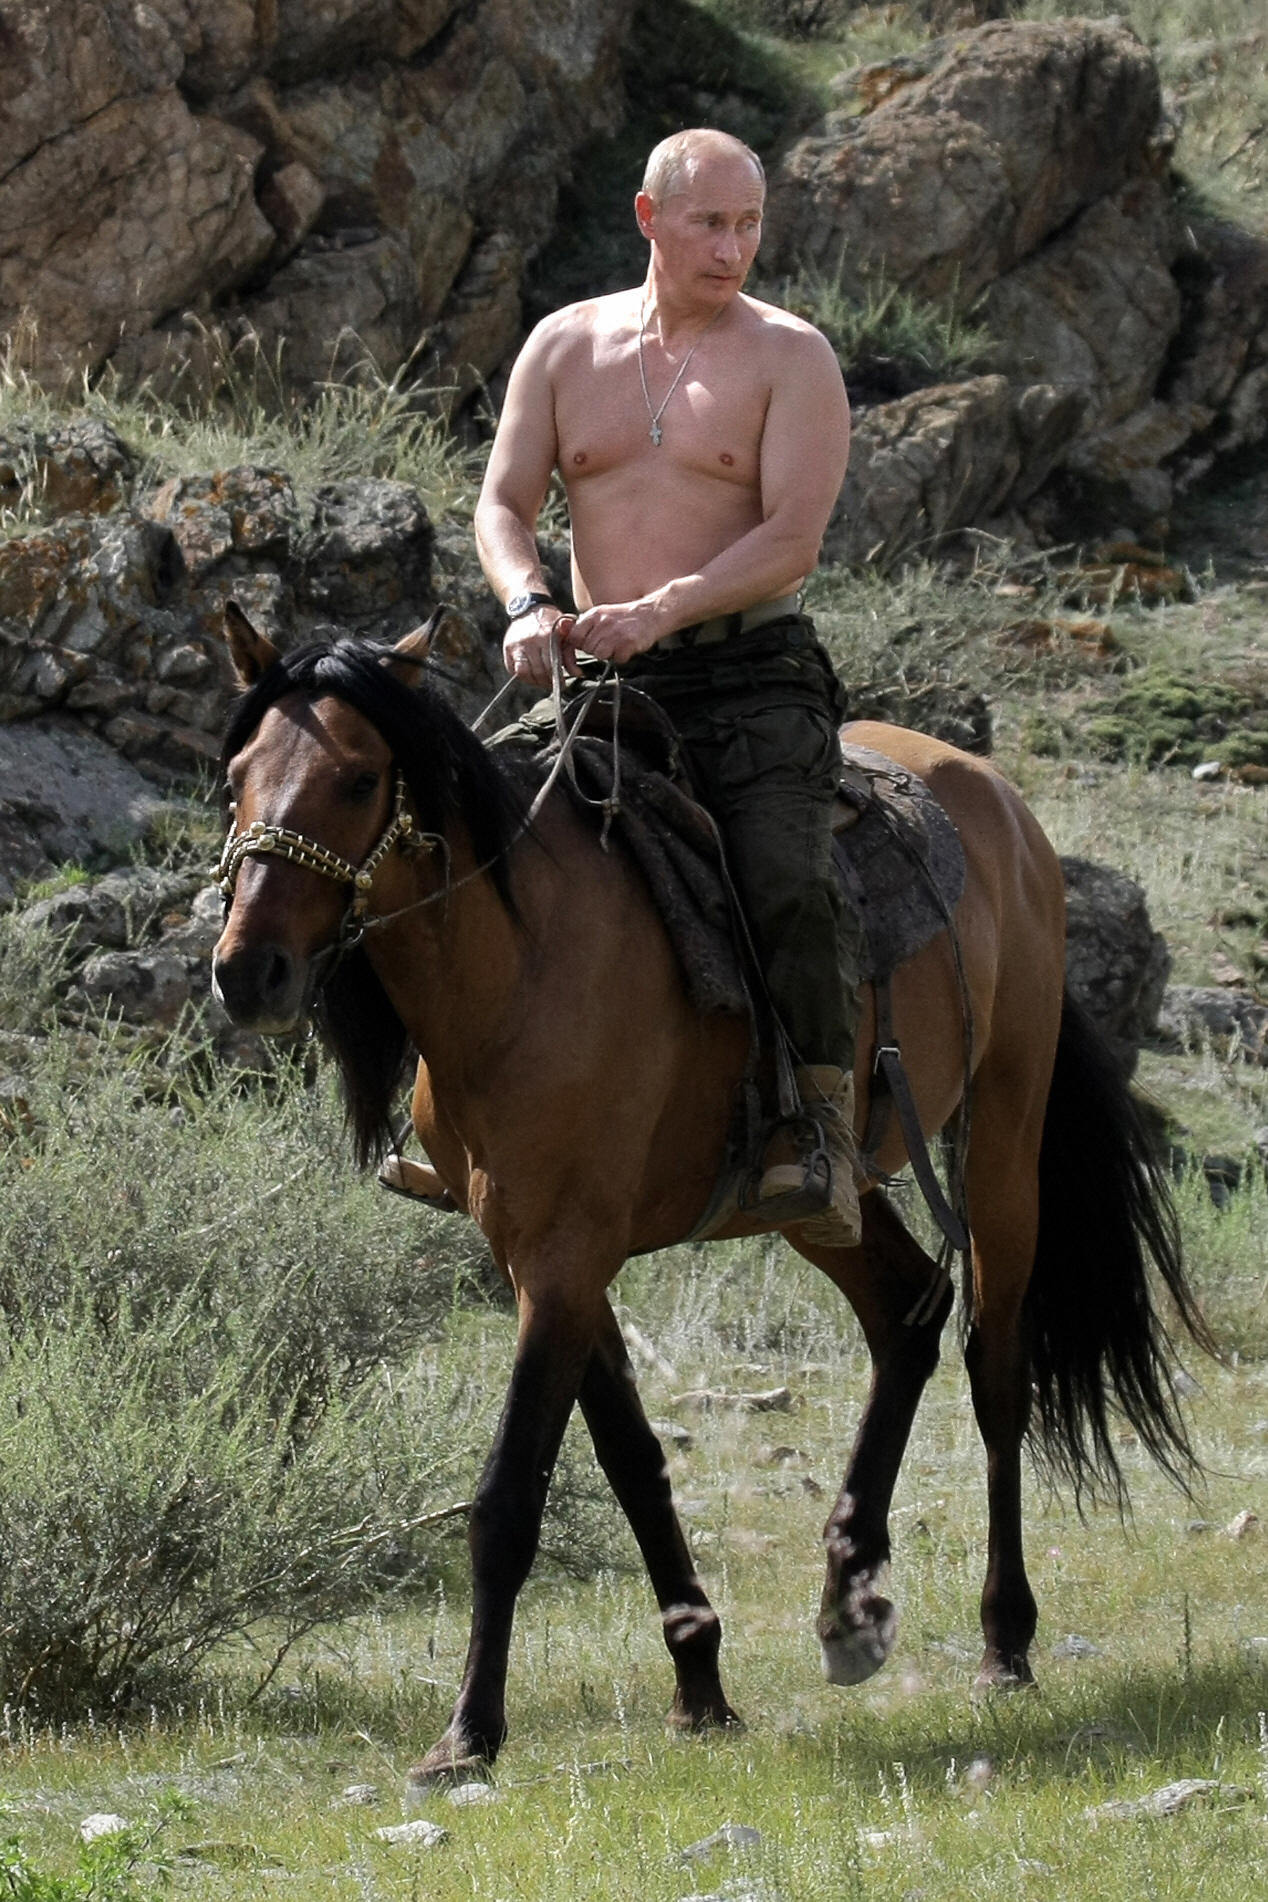
\includegraphics[height=1.7in,width=2.1in]{putin.jpg}
\end{center}
\end{frame}

\begin{frame}{Drifts vs Shifts}
Data can change gradually (drift) or suddenly (shift or switch). \newline\newline
Example - targeted advertisement:
\begin{itemize}
\item Gradual drift -  person's new skiing hobby effect on advertisement algorithms 
\item  Sudden Switch (shift)  - person's engagement effect on advertisement algorithms 
\end{itemize}
\begin{center}
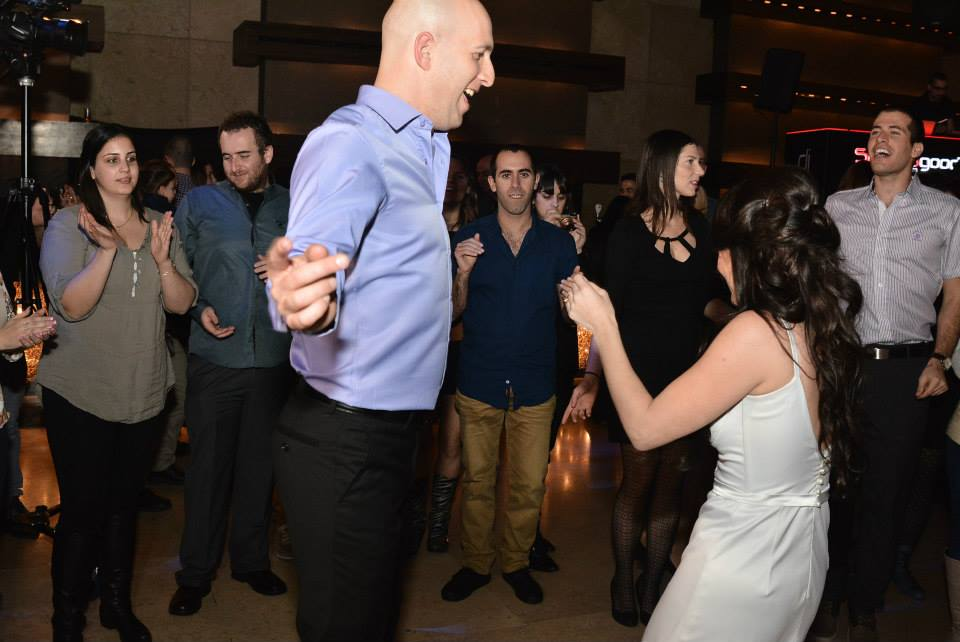
\includegraphics[height=1.7in,width=2.1in]{haim.jpg}
\end{center}
\end{frame}

\begin{frame}{Suggested Method}
\begin{itemize}
\item Use selective sampling to detect switch\newline
\item Exploit notion of confidence provided by selective sampling\newline
\item Avoid unnecessary loss of information while overcoming switch effect\newline
\item Time windows used for change detection but not for classification\newline
\end{itemize}
\end{frame}

\begin{frame}{Expected Objectives}
Approaching the problem of shifting concept in an on-line learning classification or regression setting, using selective sampling principles to overcome switch, the following objectives are set:\newline
\begin{enumerate}
\item Detect the switch\newline
\item If switch is undetected - assure that the harm caused by the switch is minor\newline
\item Small probability for false detections
\end{enumerate}
\end{frame}


\section{Classification Analysis}




\begin{frame}{Problem Setting - On-line Classification}
Problem setup:\newline
\begin{itemize}
\item $\vxi{t}\in R^d$\newline
\item $y_t\in\{\pm1\}$\newline
\end{itemize}
Assumptions:\newline
\begin{itemize}
\item $\|\vxi{t}\|=\|\vu\|=\|\vv\|=1$, $\vu,\vv\in R^d$ \newline
\item For $t\leq\tau$ holds $\Exp{y_t}=\vut\vxi{t}$\newline
\item For $t>\tau$ holds $\Exp{y_t}=\vvt\vxi{t}$
\end{itemize}
\end{frame}

\begin{frame}{Problem Setting}
\begin{itemize}
\item At each round $t$ instance $\vxi{t}$ is observed\newline
\item Prediction $\hat{y}_t$ is issued\newline
\item Regret $R_t$ is suffered\newline
\item True label $y_t$ can be queried \newline
\end{itemize}
Linear classification is used to issue prediction:
\begin{equation}
\hat{y}_t=\sign\left\{\vwti{t}\vxi{t}\right\}
\end{equation}
\end{frame}

\begin{frame}{RLS Estimator}
$\vwi{t}$ would be the RLS estimator (Chesa-Bianchi at all. 2004, 2006, 2009) solving the following problem:\newline\newline
\begin{equation}
\vwi{t}=\min_{\vw\in R^d}{\left\{\sum\limits_{i=1}^{n}\left(y_i-\vwt\vxi{i}\right)^2+\|\vw\|^2\right\}}
\label{RLS_prob}
\end{equation}\newline\newline
with $n=N_t$ being the number of queries issued until round $t-1$
\end{frame}

\begin{frame}{RLS Estimator}
The solution to equation \ref{RLS_prob} is:\newline\newline
\begin{equation}
\vwi{t}=\left(I+S_{t-1}S_{t-1}^T+ \vxi{t} \vxti{t}\right)^{-1}S_{t-1}Y_{t-1}
\label{RLS}
\end{equation}
\newline
Where:\newline
\begin{itemize}
\item $S_{t-1}=(\vxi{1},...,\vxi{n})\in R^{d\times n}$ \newline
\item $Y_{t-1}=(y_1,...,y_n)\in R^n$.
\end{itemize}
\end{frame}

\begin{frame}{RLS Estimator}
Equivalent formulation:
\begin{equation}
\vwi{t}=A_{t}^{-1}b_t
\label{RLS2}
\end{equation}
Where:\newline
\begin{itemize} 
\item $A_t=\left(I+\sum\limits_{i=1}^{n}\vxi{i} \vxti{i}+ \vxi{t} \vxti{t}\right)\in R^{d\times d}$\newline
\item $b_t=\sum\limits_{i=1}^{n}y_i\vxi{i}\in R^d$ \newline
\end{itemize}
$A_t$ can be viewed as covariance or "confidence " matrix
\end{frame}

\begin{frame}{BBQ Algorithm - Querying Labels}
Cesa-Bianchi, Gentile, Orabona 2009:
\newline\newline
Selective sampling algorithm -\newline
\begin{itemize}
\item Set $\kappa\in\left(0,1\right)$\newline
\item Calculate $r_t=\vxti{t}A_{t}^{-1}\vxi{t}$\newline
\item  If $r_t> t^{-\kappa}$ label $y_t$ is queried\newline
\item If $r_t\leq t^{-\kappa}$  label $y_t$ remains unknown
\end{itemize}
\end{frame}

\begin{frame}{RLS Estimator and  BBQ Algorithm Properties}
Assuming standard, no switch setting, $\left(\vu=\vv\right)$:\newline
\begin{itemize}
\item Logarithmic cumulative regret $R_T$:
\begin{equation}
 R_T\leq O\left(d\ln{T}\right)
\end{equation}
\item Reduced number of queried labels $N_T$:
\begin{equation}
N_T\sim O\left(dT^{\kappa}\ln{T}\right)
\end{equation}
\item Controlled estimator bias $B_t$:
\begin{equation}
B_t=\vwti{t}\vxi{t}-\Exp{\vwti{t}\vxi{t}}\leq r_t+\sqrt{r_t}
\end{equation}
\end{itemize} 
\end{frame}


\begin{frame}{Effect of Switch}
\begin{itemize}
\item Switch from $\vu$ to $\vv$ at round $\tau$ increases bias bound:\newline
\newline
\begin{equation}
B_t\leq r_t+\sqrt{r_t}+N_{\tau}\|\vv-\vu\|\sqrt{r_t}
\end{equation}\newline
\item The bias $B_t$ controls the regret $R_T$. So switch at round $\tau$ increases regret bound:\newline\newline
\begin{equation}
 R_T\leq O\left(\left\{\|\vv-\vu\|^2{\tau}^{2\kappa}\left(d\ln{\tau}\right)^2+1\right\}d\ln{T}\right)
\end{equation}
\end{itemize}
\end{frame}

\begin{frame}{Using Selective Sampling to Detect Switch}
\begin{itemize}
\item When switch occurs low cumulative regret can no longer be expected \newline
\item Selective sampling approach measures estimator's confidence regarding prediction on give instance $\vxi{t}$ \newline
\item When confidence on instance $\vxi{t}$ is high prediction should be close to optimal \newline
\item Evaluating prediction on "high confidence" instances can be used to detect change \newline
\end{itemize}


\end{frame}

\begin{frame}{Using Selective Sampling to Detect Switch}
Confidence factor $r_t=\vxti{t}A_{t}^{-1}\vxi{t}$ :\newline
\begin{itemize}
\item Small  $r_t$ - high confidence regarding instance $\vxi{t}$
\item Large  $r_t$ - high uncertainty (low confidence) regarding instance $\vxi{t}$
\newline
\end{itemize}
 $r_t$ controls both the bias $B_t$  and the instantaneous regret $R_t$:\newline
\begin{itemize}
\item If $r_t$ is large, low regret $R_t$ can not be assured, switch or no switch.
\item If $r_t$ is small, low regret $R_T$ should be expected. Unless a switch had occurred...
\end{itemize}

\end{frame}


\begin{frame}{Using Selective Sampling to Detect Switch}
 Main idea - evaluate performance on instances with small $r_t$ to detect switch.\newline\newline
Bad performance will indicate that switch had occurred.\newline
\begin{itemize}
\item Performance cannot be evaluated comparing prediction $\hat{y}_t$ to label $y_t$ due to noise\newline
\item Even if optimal classifier $\vv$ is known - error probability will be  $\frac{1-\left|\vvt\vxi{t}\right|}{2}$\newline
\item Prediction will be evaluated comparing to optimal classifier $\left\vert\vwti{t}\vxi{t}-\vvt\vxi{t}\right\vert$\newline
\end{itemize}
\end{frame}



\begin{frame}{Windowed Demo Classifiers}
\begin{itemize}
\item Problem - optimal classifier $\vv$ is unknown.\newline
\item Solution - estimate optimal classifier $\vv$ with demo classifier $h_t$. \newline
\item Demo classifier $h_t$  constructed from a window of last $L$ rounds and should estimate $\vv$ well enough \newline
\item Performance of $\vwi{t}$ comparing to $h_t$ will evaluate $\left\vert\vwti{t}\vxi{t}-\vvt\vxi{t}\right\vert$ and indicate possible switch
\end{itemize}
\end{frame}


\begin{frame}{Construction of Windowed Demo Classifier}
\begin{itemize}
\item Parameter - initial window length $L_0>0$ \newline
\item Calculate window length $L_t=L_0+\sqrt{t}$\newline
\item At round $t$  select a window of last $L_t$ instances  \newline
\item Calculate $A_{L_t}=\left(I+\sum\limits_{l=t-L_t}^{t-1}{\vxi{l}\vxti{l}}\right), b_{L_t}=\sum\limits_{l=t-L_t}^{t-1}y_l\vxi{l}$ \newline
\item Construct demo classifier $h_t=\left(A_{L_t}+\vxi{t}\vxti{t}\right)^{-1}b_{L_t}$
\end{itemize}
\end{frame}

\begin{frame}{Resolution of Windowed Demo Classifier}

\begin{itemize}
\item Demo classifier $h_t$ constructed at round $t$ from a window of last $L_t$ instances\newline
\item Demo classifier $h_t$ will be used to evaluate next  $KL_t$ instances\newline
\item Next demo classifier $h_{t_next}$ will be constructed at round $KL_t+1$\newline
\item Only $\frac{T}{K}$ labels will be queried\newline
\item Switch detection resolution reduced from $L_t$ to $KL_t$
\end{itemize}

\end{frame}


\begin{frame}{Algorithm for Detecting Switch}

\begin{itemize}
\item Calculate estimator $\vwi{t}=A_{t}^{-1}b_t$ \newline
\begin{itemize}
\item Where $A_t=\left(I+\sum\limits_{i=1}^{N_t}\vxi{i} \vxti{i}+ \vxi{t} \vxti{t}\right), b_t=\sum\limits_{i=1}^{N_t}y_i\vxi{i}$\newline\newline
\end{itemize}
\item Calculate demo classifier $h_t=\left(A_{L_t}+\vxi{t}\vxti{t}\right)^{-1}b_{L_t}$ \newline
\begin{itemize}
\item $A_{L_t}=\left(I+\sum\limits_{l=m_t-L_t}^{m_t}{\vxi{l}\vxti{l}}\right), b_{L_t}=\sum\limits_{l=m_t-L_t}^{m_t}y_l\vxi{l}$ \newline\newline
\end{itemize}
\item Calculate $r_t=\vxti{t}A_{t}^{-1}\vxi{t}$\newline
\item Calculate $r_{L_t}=\vxti{t}\left(A_{L_t}+\vxi{t}\vxti{t}\right)^{-1}\vxi{t}$
\end{itemize}
\end{frame}

\begin{frame}{Algorithm for Detecting Switch}
\begin{itemize}
\item Parameter - $\delta\in\left(0,1\right)$\newline
\item Calculate $\delta_t=\frac{\delta}{t(t+1)}$\newline
\item Calculate $C_t=\left\vert\vwti{t}\vxi{t}-h_{t}^{\top}\vxi{t}\right\vert$\newline
\item Calculate:\newline\newline $K_t=\left(\sqrt{2\ln{\frac{2}{\delta_t}}}+1\right)\sqrt{r_t}+r_t+\left(\sqrt{2\ln{\frac{2}{\delta_t}}}+1\right)\sqrt{r_{L_t}}+r_{L_t}$\newline
\item If $C_t>K_t$ declare switch and restart classifier $w_t$ from zero. Else continue to next round
\end{itemize}
\end{frame}

\begin{frame}{Algorithm's Main Result}
\begin{itemize}
\item If $C_t>K_t$ \newline
\begin{itemize}
\item If switch occurred it is detected  \newline
\item If no switch occurred $\pr{C_t>K_t}\leq \left(1-2\delta\right)$ - to be proved  \newline
\end{itemize}
\item If $C_t\leq K_t$ \newline
\begin{itemize}
\item If no switch occurred, no change applied to standard setting   \newline
\item If a switch occurred and undetected as $C_t\leq K_t$, additional regret caused would be small - to be proved   \newline 
\end{itemize}
\end{itemize}
\end{frame}

\begin{frame}{Algorithm's Main Result}
Main result:\newline\newline
\begin{enumerate}
\item If a switch occurs - algorithm detects it, or assures it causes small harm\newline 
\item No switch occurs - no false detection
\end{enumerate}
\end{frame}

\begin{frame}{Proving Main Result}
Proof structure as follows:\newline
\begin{enumerate}
\item Proving undetected switch will cause low regret:\newline
\begin{itemize}
\item Bounding instantaneous regret \newline
\item Summing to cumulative regret \newline
\end{itemize}
\item Proving probability for false positives is small
\end{enumerate}
\end{frame}

\begin{frame}{Proving Main Result - Instantaneous Regret Bound}
Instantaneous regret $R_t$ controlled by the term $|\vwti{t}\vxi{t}-\vvt\vxi{t}|$:
\begin{eqnarray}
&&R_t=\pr{y_t\vwti{t}\vxi{t}<0}-\pr{y_t\vvt\vxi{t}<0}\leq\nonumber\\
&&\varepsilon I_{\{\left|\vvt\vxi{t}\right|<\varepsilon\}}+\pr{\left|\vwti{t}\vxi{t}-\vvt\vxi{t}\right|\geq\varepsilon}
\label{regret_wt_ht1}
\end{eqnarray}
$|\vwti{t}\vxi{t}-\vvt\vxi{t}|$ can be bounded by triangle inequality:
\begin{eqnarray}
&&\left\vert\vwti{t}\vxi{t}-\vvt\vxi{t}\right\vert\leq\left\vert\vwti{t}\vxi{t}-h_{t}^{\top}\vxi{t}\right\vert+\left\vert\vvti{t}\vxi{t}-h_{t}^{\top}\vxi{t}\right\vert\nonumber\\
&&=C_t+\left\vert\vvti{t}\vxi{t}-h_{t}^{\top}\vxi{t}\right\vert
\label{triangl_ht_wt}
\end{eqnarray}
\end{frame}

\begin{frame}{Proving Main Result - Instantaneous Regret Bound}
\begin{itemize}
\item $C_t$ is bounded by $K_t$ as a switch was not detected:
\begin{equation}
C_t\leq K_t=\left(\sqrt{2\ln{\frac{2}{\delta_t}}}+1\right)\sqrt{r_t}+r_t+\left(\sqrt{2\ln{\frac{2}{\delta_t}}}+1\right)\sqrt{r_{L_t}}+r_{L_t} 
\end{equation}
\item From properties of RLS estimator (Cesa-Bianchi at all) applied to demo classifier $h_t$:
\begin{equation}
\left\vert\vvt\vxi{t}-h_{t}^{\top}\vxi{t}\right\vert\leq\left(\sqrt{2\ln{\frac{2}{\delta_t}}}+1\right)\sqrt{r_{L_t}}+r_{L_t}
\label{rLt_false}
\end{equation}
With probability $1-\delta_t$.
\end{itemize}
\end{frame}



%\begin{frame}{Proving Main Result - Instantaneous Regret Bound}
%\begin{itemize}
%\item Combining bounds on $C_t$ and on $\left\vert\vvt\vxi{t}-h_{t}^{\top}\vxi{t}\right\vert$:
%\begin{eqnarray}
%&&\left\vert\vwti{t}\vxi{t}-\vvt\vxi{t}\right\vert\leq\sqrt{r_t}\left(\sqrt{2\ln{\frac{2}{\delta_t}}}+1\right)+r_t\nonumber\\
%&&+2\sqrt{r_{L_t}}\left(\sqrt{2\ln{\frac{2}{\delta_t}}}+1\right)+2r_{L_t}
%\label{triangl_ht_wt2}
%\end{eqnarray}
%\item Using identities $\pr{A}=\Exp{I_A}$, and $I_{\{x<1\}}\leq e^{1-x}$:
%\begin{eqnarray}
%&&\pr{\left|\vwti{t}\vxi{t}-\vvt\vxi{t}\right|\geq\varepsilon}\leq 2\exp\left\{1-\frac{\alpha_{\varepsilon,t}}{r_{L_t}}\right\}\\
%&&+2\exp\left\{1-\frac{\beta_{\varepsilon}}{r_{L_t}}\right\}+\exp\left\{1-\frac{\alpha_{\varepsilon,t}}{r_t}\right\}+\exp\left\{1-\frac{\beta_{\varepsilon}}{r_t}\right\}\nonumber
%\label{exponent_regret_class}
%\end{eqnarray}
%\end{itemize}
%\end{frame}


\begin{frame}{Proving Main Result - Instantaneous Regret Bound}

Combining bounds on $C_t$ and on $\left\vert\vvt\vxi{t}-h_{t}^{\top}\vxi{t}\right\vert$:
\begin{eqnarray}
&&\left\vert\vwti{t}\vxi{t}-\vvt\vxi{t}\right\vert\leq\sqrt{r_t}\left(\sqrt{2\ln{\frac{2}{\delta_t}}}+1\right)+r_t\nonumber\\
&&+2\sqrt{r_{L_t}}\left(\sqrt{2\ln{\frac{2}{\delta_t}}}+1\right)+2r_{L_t}
\label{triangl_ht_wt2}
\end{eqnarray}

\end{frame}


\begin{frame}{Proving Main Result - Instantaneous Regret Bound}
Using identities:\newline
\begin{itemize}
\item $\pr{A}=\Exp{I_A}$
\item $I_{\{x<1\}}\leq e^{1-x}$\newline
\end{itemize}
final bound instantaneous regret $R_t$ achieved:
\begin{eqnarray}
&&R_t\leq\varepsilon I_{\{\left|\vvt\vxi{t}\right|<\varepsilon\}}+ \pr{\left|\vwti{t}\vxi{t}-\vvt\vxi{t}\right|\geq\varepsilon}\\
&&\leq\varepsilon I_{\{\left|\vvt\vxi{t}\right|<\varepsilon\}}+ 2\exp\left\{1-\frac{\alpha_{\varepsilon,t}}{r_{L_t}}\right\}+2\exp\left\{1-\frac{\beta_{\varepsilon}}{r_{L_t}}\right\}\nonumber\\
&&+\exp\left\{1-\frac{\alpha_{\varepsilon,t}}{r_t}\right\}+\exp\left\{1-\frac{\beta_{\varepsilon}}{r_t}\right\}+\delta_t\nonumber
\label{exponent_regret_class}
\end{eqnarray}
\end{frame}

%Definition:
%\begin{itemize}
%\item $\alpha_{\varepsilon,t}}=\frac{\varepsilon^2}{36\left(\sqrt{2\ln{\frac{2}{\delta_t}}}+1\right)^2}\right\}$
%\item $beta_{\varepsilon}=\frac{\varepsilon}{6}$
%\end{itemize}


\begin{frame}{Proving Main Result - Cumulative Regret Bound}
Cumulative regret $R_T$ is given by:
\begin{equation}
R_T=\sum\limits_{t=1}^{T}R_t
\label{cum_reg_define}
\end{equation}
Cumulative regret $R_T$ will be bounded by summing over bound of instantaneous regret $R_t$. \newline\newline Calculation outline:\newline
\begin{enumerate}
\item Summation over the $r_t$ terms - separate calculation for:
\begin{itemize}
\item Rounds $t$ for which with $r_t\leq t^{-\kappa}$
\item Rounds $t$ for which with $r_t> t^{-\kappa}$
\end{itemize}
\item Summation over the $r_{L_t}$ terms.
\item Deriving final bound
\end{enumerate}
\end{frame}

\begin{frame}{Proving Main Result - Cumulative Regret Bound}
Summation over $r_t$ terms - for rounds with $r_t> t^{-\kappa}$ - \newline
\begin{itemize}
\item Identity $\exp\{-x\}\leq\frac{1}{ex}$ gives:
\begin{eqnarray}
&&\sum\limits_{t=T_1,r_t> t^{-\kappa}}^{T}\exp\left\{1-\frac{\alpha_{\varepsilon,t}}{r_t}\right\}\leq \frac{1}{\alpha_{\varepsilon,T}}\sum\limits_{t=T_1,r_t> t^{-\kappa}}^{T}r_t\nonumber
\end{eqnarray}
\item The result $ r_t\leq\left(1-\frac{\det{A_{t-1}}}{\det{A_t}}\right)$ (Cesa-Bianchi at. all 2004) yields:
\begin{eqnarray}
&&\frac{1}{\alpha_{\varepsilon,t}}\sum\limits_{t=T_1,r_t> t^{-\kappa}}^{T}r_t\leq\frac{1}{\alpha_{\varepsilon,t}}\sum\limits_{t=T_1,r_t> t^{-\kappa}}^{T}\left(1-\frac{\det{A_{t-1}}}{\det{A_t}}\right)\nonumber
\end{eqnarray}
\end{itemize}
\end{frame}

\begin{frame}{Proving Main Result - Cumulative Regret Bound}
Summation over $r_t$ terms - for rounds with $r_t> t^{-\kappa}$ - \newline
\begin{itemize}
\item Identity $1-x\leq -\ln{x}$ (for $x\leq1$) gives:
\begin{eqnarray*}
\frac{1}{\alpha_{\varepsilon,t}}\sum\limits_{t=T_1,r_t> t^{-\kappa}}^{T}\left(1-\frac{\det{A_{t-1}}}{\det{A_t}}\right)\leq -\frac{1}{\alpha_{\varepsilon,t}}\sum\limits_{t=T_1,r_t> t^{-\kappa}}^{T}\ln{\left(\frac{\det{A_{t-1}}}{\det{A_t}}\right)}
\end{eqnarray*}
\item Computing the sum will give final expression:
\begin{eqnarray*}
 -\frac{1}{\alpha_{\varepsilon,t}}\sum\limits_{t=T_1,r_t> t^{-\kappa}}^{T}\ln{\left(\frac{\det{A_{t-1}}}{\det{A_t}}\right)}\leq \frac{1}{\alpha_{\varepsilon,t}}\left\{d\ln{T}- \ln\left(\det{A_{T_1}}\right)\right\}
\end{eqnarray*}
\end{itemize}
\end{frame}

\begin{frame}{Proving Main Result - Cumulative Regret Bound}
Summation over $r_t$ terms - for rounds with $r_t\leq t^{-\kappa}$ - \newline
\begin{itemize}
\item Substituting  $r_t\leq t^{-\kappa}$ and replacing sum with integral yields:  
\begin{eqnarray}
&&\sum\limits_{t=T_1,r_t> t^{-\kappa}}^{T}\exp\left\{1-\frac{\alpha_{\varepsilon,t}}{r_t}\right\}\leq e\sum\limits_{t=T_1,r_t> t^{-\kappa}}^{T}\exp\left\{-\frac{\alpha_{\varepsilon,t}}{t^{-\kappa}}\right\}\nonumber\\
&&\leq e\int_{T_1}^{T}\nonumber\exp\left\{-\alpha_{\varepsilon,T}t^{\kappa}\right\}\,dt=\nonumber\\
&&=\frac{e}{\kappa\left(\alpha_{\varepsilon,T}\right)^{\frac{1}{\kappa}}}\left(\Gamma\left\{\frac{1}{\kappa},\alpha_{\varepsilon,T}T_{1}^{\kappa}\right\}-\Gamma\left\{\frac{1}{\kappa},\alpha_{\varepsilon,T}T^{\kappa}\right\}\right)\nonumber
\end{eqnarray}
\item Last equality follows from the identity:
\begin{equation}
\int\exp\{az^s\}\,dz=-\frac{z(-az^s)^{-\frac{1}{s}}}{s}\Gamma\left\{\frac{1}{s},-az^s\right\}
\label{incomplete_gamma}
\end{equation}
\end{itemize}
\end{frame}

\begin{frame}{Proving Main Result - Cumulative Regret Bound}
Summation over $r_{L_t}$ terms - \newline\newline
Matrix Chernoff bound - for a series of random, i.i.d PSD matrices $Z_k\in R^{d\times d}$ holds:
\begin{equation}
\pr{\lambda_{\min}\left\{\sum_k Z_k \right\}\leq \left(1-\gamma\right)\mu_{\min}}\leq d\left(\frac{e^{-\gamma}}{ \left(1-\gamma\right)^{ \left(1-\gamma\right)}}\right)^{\frac{\mu_{\min}}{\rho}}
\end{equation}
where:
\begin{itemize}
\item $\gamma\in (0,1)$
\item $\mu_{\min}=\lambda_{\min}\left\{\sum_k\Exp{Z_k}\right\}$
\item $\lambda_{\max}\left\{\Exp{Z_k}\right\}\leq\rho$
\end{itemize}

\end{frame}


\begin{frame}{Proving Main Result - Cumulative Regret Bound}
Summation over $r_{L_t}$ terms - \newline
\begin{itemize}
\item Assumption: smallest eigenvalue of covariance matrix grows linearly - $\lambda_{\min}\left\{\sum\limits_{k=1}^{L}\Exp{\vxi{k}\vxti{k}}\right\}\sim O\left(\frac{L}{d}\right)$\newline 
\item Using Chernoff matrix bound on $Z_k=\vxi{k}\vxti{k}$, under the above assumption, yields:
\begin{equation}
\lambda_{\min}\left\{A_{L_t}\right\}=\lambda_{\min}\left\{I+\sum\limits_{k=1}^{L_t} \vxi{k}\vxti{k}\right\}>(1-\gamma)\frac{L_t}{d}+1
\label{lamda_min_bound}
\end{equation}
\end{itemize}
\end{frame}


\begin{frame}{Proving Main Result - Cumulative Regret Bound}
Summation over $r_{L_t}$ terms - \newline\newline
Using the bound and identities below:\newline
\begin{itemize}
\item For unit normed $\vx$: $\vxt M\vx\leq \lambda_{max}\{M\}$
\item $\lambda_{max}\left\{M\right\}=\frac{1}{\lambda_{min}\left\{M^{-1}\right\}}$
\item $\lambda_{\min}\left\{A_{L_t}\right\}>\left(1-\gamma\right)\frac{L_t}{d}$\newline
\end{itemize}
we get:
\begin{eqnarray}
r_{L_t}=\vxti{t}\left(A_{L_t}+\vxi{t}\vxti{t}\right)^{-1}\vxi{t}\leq\frac{d}{\left(L_t+2\right)\left(1-\gamma\right)}
\end{eqnarray}
\end{frame}


\begin{frame}{Proving Main Result - Cumulative Regret Bound}
Summation over $r_{L_t}$ terms - \newline\newline
\begin{itemize}
\item Replacing $L_t=L_0+\sqrt{t}$ into the bound would yield:
\begin{eqnarray}
r_{L_t}\leq\frac{d}{\left(L_0+\sqrt{t}+2\right)\left(1-\gamma\right)}
\end{eqnarray}
\item Substituting bound $r_{L_t}$ into the sum over regret $R_T$ bound: 
\begin{eqnarray*}
&&\sum\limits_{t=T_1}^{T}\exp\left\{1-\frac{\alpha_{\varepsilon,t}}{r_{L_t}}\right\}\leq e\sum\limits_{t=T_1,r_t> t^{-\kappa}}^{T}\exp\left\{-\hat{\alpha}_{\varepsilon,t}\left(L_0+\sqrt{t}\right)\right\}\nonumber\\
\end{eqnarray*}
\end{itemize}
\end{frame}



\begin{frame}{Proving Main Result - Cumulative Regret Bound}
Summation over $r_{L_t}$ terms - \newline\newline
Now replacing sum with integral and solving as before yields:
\begin{eqnarray*}
&&e\sum\limits_{t=T_1}^{T}\exp\left\{-\hat{\alpha}_{\varepsilon,t}\left(L_0+\sqrt{t}\right)\right\}\leq\\
&&\frac{2e}{\left(\tilde{\alpha}_{\varepsilon,T}\right)^{2}}\left(\Gamma\left\{2,\tilde{\alpha}_{\varepsilon,T}\left(T_{1}-L_0\right)^{\frac{1}{2}}\right\}-\Gamma\left\{2,\tilde{\alpha}_{\varepsilon,T}\left(T-L_0\right)^{\frac{1}{2}}\right\}\right)\nonumber
\end{eqnarray*}
\end{frame}


\begin{frame}{Proving Main Result - Cumulative Regret Bound}
\begin{itemize}
\item Summing all developed bounds yields:
\begin{equation}
 R_T\leq O\left(d\left\{\ln{T}\right\}^2\right)
\end{equation}
\item Cumulative regret controlled and small\newline
\item Bound overcomes switch effect - square logarithmic bound in T comparing to more than linear bound in $\tau$
\end{itemize}

\end{frame}



%
%\begin{frame}{Proving Main Result - Cumulative Regret Bound}
%\begin{itemize}
%\item Summing all developed bounds yields:
%\begin{equation}
% R_T\leq O\left(d\left\{\ln{T}\right\}^2\right)
%\end{equation}
%\item Cumulative regret controlled and small\newline
%\item Bound overcomes switch effect
%\end{itemize}
%
%\end{frame}



\begin{frame}{Proving Main Result - No False Positives}
\begin{itemize}
\item Reminder -switch detection if $C_t>K_t$\newline
\item Assuring no false detection - if no switch occurs than $C_t\leq K_t$\newline
\item From triangle inequality:
\begin{equation}
C_t=\left\vert\vwti{t}\vxi{t}-h_{t}^{\top}\vxi{t}\right\vert\leq\left\vert\vwti{t}\vxi{t}-\vvt\vxi{t}\right\vert+\left\vert\vvt\vxi{t}-h_{t}^{\top}\vxi{t}\right\vert
\end{equation}
\end{itemize}
\end{frame}




\begin{frame}{Proving Main Result - No False Positives}
\begin{itemize}
\item Reminder - from RLS estimator properties, holds with probability $1-2\delta_t$:\newline
\begin{itemize}
\item $\left\vert\vwti{t}\vxi{t}-\vvt\vxi{t}\right\vert\leq\sqrt{r_t}\left(\sqrt{2\ln{\frac{2}{\delta_t}}}+1\right)+r_t$\newline
\item $\left\vert\vvt\vxi{t}-h_{t}^{\top}\vxi{t}\right\vert\leq\left(\sqrt{2\ln{\frac{2}{\delta_t}}}+1\right)\sqrt{r_{L_t}}+r_{L_t}$\newline
\end{itemize}
\item Substituting this into bound:
\begin{eqnarray*}
&&C_t\leq\sqrt{r_t}\left(\sqrt{2\ln{\frac{2}{\delta_t}}}+1\right)+r_t\\
&&+\left(\sqrt{2\ln{\frac{2}{\delta_t}}}+1\right)\sqrt{r_{L_t}}+r_{L_t}\leq K_t
\end{eqnarray*}
\end{itemize}
\end{frame}

\begin{frame}{Proving Main Result - No False Positives}
\begin{itemize}
\item Last result assures that if no switch occurred $C_t\leq K_t$ with probability $1-2\delta_t$\newline
\item Thus  the probability for a false detection at round $t$ is $2\delta_t$\newline
\item Using union bound - probability for a false detection throughout the algorithm is $2\delta$\newline


\end{itemize}
\end{frame}

\begin{frame}{Simulation Results}
Synthetic data Matlab simulation:\newline
\begin{itemize}
\item $T=10^5$, $\vxi{t}\in R^4$, $\kappa=0.7$, $L_0=500$, $K=6$
\item Instances $\vxi{t}$ drawn randomly from Gaussian distribution and then normalized
\item Labels $y_t$ drawn from Bernoulli distribution with $p_t=\frac{1-\vut\vxi{t}}{2}$\newline
\end{itemize}
Results, averaged after $100$ runs of the algorithm:\newline
\begin{itemize}
\item Optimal classifier - $28.81\%$ error
\item BBQ RLS estimator classifier - $35.76\%$ error
\item Suggested switch detection algorithm - $29.58\%$ error
\end{itemize}
\end{frame}

\begin{frame}{Simulation Results - No false Detection}
Number of switch detections, in $100$ runs of the algorithm:
\begin{center}
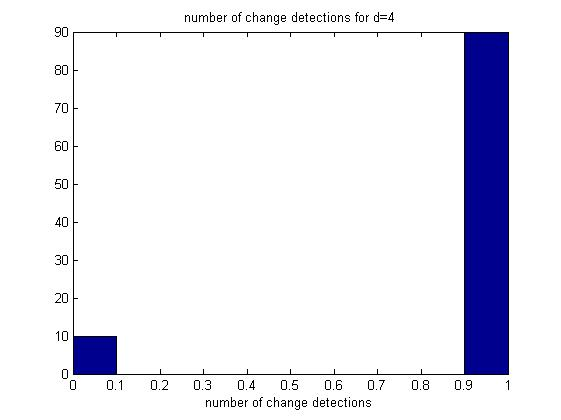
\includegraphics[height=2.5in,width=2.8in]{Ndet_clas.jpg}
\end{center}
\end{frame}

\begin{frame}{Simulation Results - Switch Detected Relatively Fast}
Distribution of switch delay, in $100$ runs of the algorithm:
\begin{center}
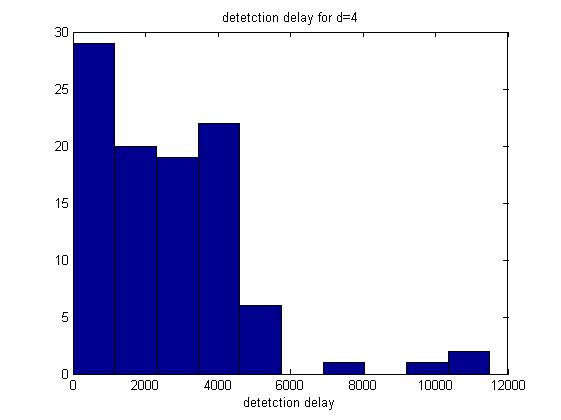
\includegraphics[height=2.5in,width=2.8in]{delay_clas.jpg}
\end{center}
\end{frame}

\section{Regression Analysis}
\begin{frame}{Problem Setting - On-line Regression}
\begin{itemize}
\item Analysis for regression is similar to one presented for classification.\newline
\item  Differences between the two problems will be discussed.\newline
\end{itemize}

Problem setup:

\begin{itemize}
\item $\vxi{t}\in R^d$
\item $y_t\in R$
\end{itemize}

\end{frame}


\begin{frame}{Problem Setting - On-line Regression}

Assumptions:\newline
\begin{itemize}
\item $\|\vxi{t}\|=\|\vu\|=\|\vv\|=1, \vu, \vv\in R^d$\newline
\item for $t\leq\tau$ holds:\newline\newline
 $y_t=\vut\vxi{t}+\eta_t$ and $\Exp{y_t}=\vut\vxi{t}$\newline

\item for $t>\tau$ holds:\newline\newline
 $y_t=\vvt\vxi{t}+\eta_t$ and $\Exp{y_t}=\vvt\vxi{t}$\newline
\item $\eta_t$ i.i.d noise with $\Exp{\eta_t}=0, var\left\{\eta_t\right\}=\sigma^2$ \newline
\item $\left\vert\eta_t\right\vert\leq Z_{\eta}$, $Z_{\eta}$ is known
\end{itemize}


\end{frame}

\begin{frame}{Regret Definition}
\begin{itemize}
\item Linear regression is to issue prediction:\newline
\begin{equation}
\hat{y}_t=\vwti{t}\vxi{t}
\end{equation}
\item As in classification $\vwi{t}$ is the RLS estimator: $\vwi{t}=A_{t}^{-1}b_t$\newline
\item Major difference - instantaneous regret definition:
\begin{eqnarray*}
&&R_t=\left(y_t-\hat{y}_t\right)^2-\left(y_t-\vvt\vxi{t}\right)^2\\
&&=\left(y_t-\vwti{t}\vxi{t}\right)^2-\left(y_t-\vvt\vxi{t}\right)^2\\
&&=\left(\vwti{t}\vxi{t}-\vvt\vxi{t}\right)^2-2\left(y_t-\vvt\vxi{t}\right)\left(\vwti{t}\vxi{t}-\vvt\vxi{t}\right)
\end{eqnarray*}
\end{itemize}
\end{frame}

\begin{frame}{Regret Bounds}
\begin{itemize}
\item RLS properties used to bound $\left\vert\vwti{t}\vxi{t}-\vvt\vxi{t}\right\vert$\newline
\item To bound the cumulative regret $R_T$:\newline
\begin{enumerate}
\item $\sum\limits_{t=T_1}^{T}\left(\vwti{t}\vxi{t}-\vvt\vxi{t}\right)^2$ will be bounded using RLS properties\newline  
\item Azuma's inequality will be used to bound $\sum\limits_{t=T_1}^{T}\left(y_t-\vvt\vxi{t}\right)\left(\vwti{t}\vxi{t}-\vvt\vxi{t}\right)$
\end{enumerate}
\end{itemize}
\end{frame}

\begin{frame}{Main Result for Regression}
\begin{itemize}
\item If switch occurs it is either detected or low regret assured\newline
\item In case of non detection - $R_T\leq O\left(\sqrt{d}T^{\left(1-\frac{2\kappa+1}{4}\right)}\ln{T}\right)$\newline
\item Improving expected bound due to effect of switch: $R_T\leq O\left(d^2\tau^{2\kappa}\left\{\ln{T}\right\}^2T^{1-\kappa}\right)$\newline
\item Result close to bound in no switch case - $O\left(T^{1-\kappa}\ln{T}\right)$\newline
\item Probability for false detection - $1-2\delta$\newline
\item Note - in regression problem selective sampling increases regret
\end{itemize}
\end{frame}

\begin{frame}{Simulation Results}

\end{frame}

\section{Summary}
%
%\begin{frame}{Problem}
%
%\end{frame}


\begin{frame}{Proposed Method}
\begin{itemize}
\item Problem approached - switch in data at on-line linear classification and regression settings\newline
\item Proposed solution -\newline
\begin{enumerate}
\item Using confidence notion of selective sampling for switch detection\newline
\item Constructing demo classifier $h_t$ from recent time window\newline
\item Difference between estimator and demo classifier $C_t=\left\vert\vwti{t}\vxi{t}-h_{t}^{\top}\vxi{t}\right\vert$ indicates switch\newline
\item Difference considered with respect to confidence $r_t$ about instance $\vxi{t}$
\end{enumerate}
\end{itemize}
\end{frame}


\begin{frame}{Main Results}
\begin{itemize}
\item Algorithm either detects switch or assurers low regret in case of non-detection\newline
\item Low probability for false detection\newline
\item Simulations on synthetic data results:\newline

\begin{itemize}
\item Most switches were detected in relativity short time\newline
\item Error reduced close to optimal result\newline
\item No false detections
\end{itemize}
\end{itemize}
\end{frame}


\begin{frame}{Model Limitations}
\begin{itemize}
\item Strong assumptions on instances $\vxi{t}$ distribution \newline
\item Strong assumptions on label $y_t$ distribution\newline
\item Union bound used on non independent events\newline
\item In regression setting noise bound $Z_{\eta}$ assumed to be known\newline
\item  Demo classifier construction increases number of queries \newline
\end{itemize}
\end{frame}



\begin{frame}{Future Work}
\begin{itemize}
\item Introducing proposed methods and concepts with adjustment to drift detection
\item Constructing demo classifier from recent queried labels without further sampling 
\item Weakening assumptions on data
\end{itemize}
\end{frame}

\begin{frame}{Thank You for Your Time}
Questions?
\begin{center}

\includegraphics[height=2.3in,width=2.8in]{berko.jpg}
\end{center}

\end{frame}


\end{document}